\section{32-bit addition}
\subsection{Aim}
To add two 32-bit numbers

\subsection{Code}
\begin{lstlisting}
DATA SEGMENT
	num1 DD 10000000H
	num2 DD 20000000H
	sum DD ?
DATA ENDS

CODE SEGMENT
ASSUME CS:CODE, DS:DATA
START:
	MOV AX, DATA
	MOV DS, AX
	MOV AX, [num1]
	MOV BX, [num2]
	ADD AX, BX
	MOV [sum], AX
	MOV AX, [num1+2]
	MOV BX, [num2+2]
	ADC AX, BX
	MOV [sum+2], AX
    MOV AH, 04CH
    INT 21H
CODE ENDS
END START
\end{lstlisting}

\subsection{Output}
\begin{center}
	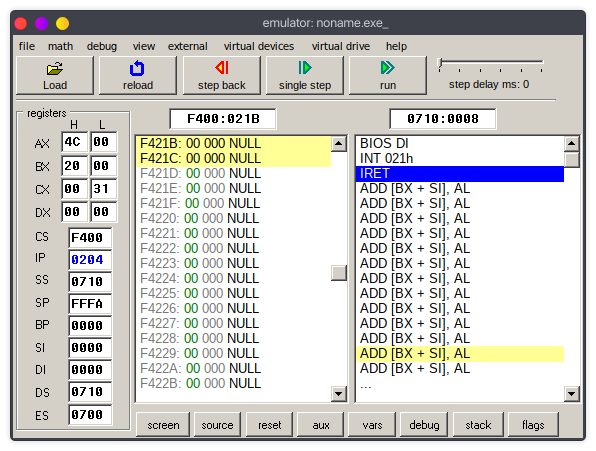
\includegraphics[width=0.90\textwidth]{img/p3/ss1.png}
	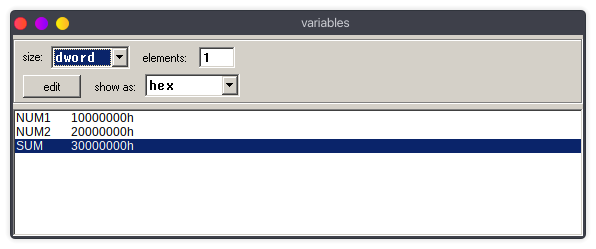
\includegraphics[width=0.90\textwidth]{img/p3/ss2.png}
\end{center}

\subsection{Result}
Two 32 bit numbers were added in emu8086 and output was verified